Durante todo el desarrollo se ha empleado la metodología ágil \textit{Scrum}. Este método se caracteriza porque se realizan entregas parciales y regulares del producto final priorizando aquellas tareas que sean de mayor importancia para el resultado deseado. El desarrollo se ejecuta en ciclos temporales cortos y de duración fija (\textit{Sprints}) y al finalizar deben proporcionar un incremento del producto que sea susceptible de ser entregado. Tras esto, se realiza una reunión con el \textit{Product Owner} para evaluar el resultado \textit{Sprint review} y se planifica la siguiente iteración (\textit{Sprint planning}).\\

\begin{figure}[h]
\centering
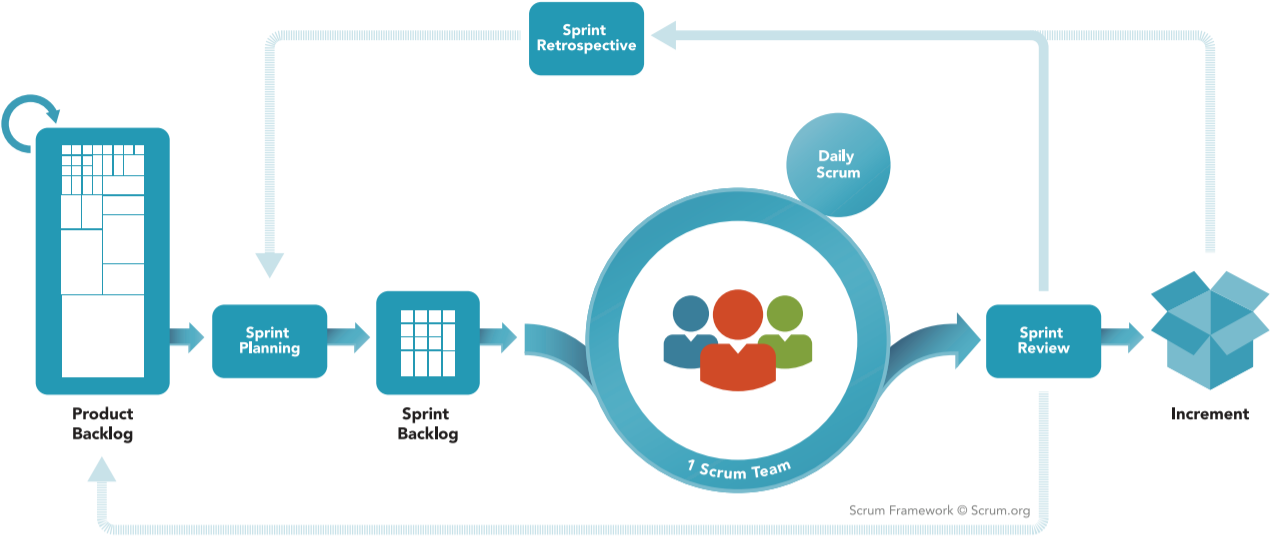
\includegraphics[scale=0.5]{../images/scrum.png} 
\caption{Metodología Scrum}
\label{fig:x scrum}
\end{figure}

Dada la naturaleza del proyecto y la poca experiencia previa en el desarrollo de chatbots esta forma de trabajar aporta la suficiente flexibilidad para subsanar los posibles errores o problemas que surjan durante el proceso de diseño o desarrollo. Por otra lado, una parte crucial en la construcción de cualquier chatbot es poder empezar a probar el servicio con usuarios reales cuando antes, de manera que se pueda ir incorporando a la base de datos toda la información recopilada y el desarrollo se pueda beneficiar de este \textit{feedback}. Es en este punto donde la entrega de valor en períodos cortos de tiempo de \textit{Scrum} es idónea para el proyecto, ya que estas iteraciones posibilitan tener una producto mínimo viable (\textit{PMI}) cuanto antes.\\

En este proyecto los \textit{Sprints} han sido de 2 semanas naturales de duración, realizando el día 14 una reunión con el \textit{Product Owner} (los tutores del proyecto) para valorar el progreso realizado y determinar las próximos pasos a seguir. \\

Por otra parte, también se ha mantenido un contacto constante a través de reuniones \textit{online} y correos electrónicos con los investigadores del Hospital General de Elche para contar en todo momento con su visto bueno en temas médicos y de diseño.\\

En los documentos anexos a este trabajo se pueden encontrar las actas de todas estas reuniones con la fecha, los participantes y los temas tratados.\\



